\documentclass[x11names,svgnames]{beamer}

\usetheme{metropolis}
\setbeamercolor{block title}{fg=LightSkyBlue4}
\usepackage{fontspec}
\usepackage[francais]{babel}
\usepackage[french, frenchkw]{algorithm2e}
\SetKwFor{Pc}{Pour chaque}{faire}{fin}
\SetKwProg{Fn}{Fonction}{:}{}
\usepackage{textcomp}
\usepackage{minted}
\usepackage{xspace}
\usepackage{amsmath}
\usepackage{mathtools}
\usepackage{marvosym}
\usepackage{tikz}
\usetikzlibrary{calc, positioning, arrows, decorations.pathmorphing}
% https://tex.stackexchange.com/questions/401884/how-do-i-change-hyperlinks-color-only
\hypersetup{
  colorlinks,
  allcolors=.,
  urlcolor=DarkBlue,
  pdftitle={AP1 - 2 décembre 2024 - La récursivité}
}


\author{}
\date{Lundi 2 décembre 2024}

\title{
\includegraphics[width=0.75\textwidth]{../../../img/logo-igm.png} \\ Algorithmique et Programmation 1}
\institute{L1 Mathématiques - L1 Informatique \\ Semestre 1}

\begin{document}

\maketitle

\section{Retour sur les fonctions}

\begin{frame}
  \begin{block}{Fonction}
    \vspace{0pt}
    En informatique, une fonction est :
    \begin{itemize}
    \item Un morceau de programme
    \item Portant en général \emph{un nom}
    \item Prenant un ou plusieurs \emph{paramètres} (ou zéro)
    \item Renvoyant un résultat (la plupart du temps)
    \end{itemize}
  \end{block}
\end{frame}

\begin{frame}{Fonctions}
    \begin{tikzpicture}
      % Rectangle pour représenter la fonction
      \node [draw, rectangle, text width=2cm, minimum height=1.5cm, align=center] (function) at (0,0) {Fonction};

      % Chemin pour représenter l'entrée (paramètres)
      \draw[-latex] (-5,0) -- (-1.2,0) node[midway, above, label={below: (paramètres)}] {Entrée};

      % Chemin pour représenter la sortie (valeur de retour)
      \draw[-latex] (1.2,0) -- (5,0) node[midway, above, label= {below: (valeur de retour)}] {Sortie};

      % Flèche d'affichage (zig-zag)
      \onslide<2->{\draw [decorate, -latex, decoration={snake, segment length=5mm, amplitude=1mm, post length=1mm}] (0,0.5) -- (0,2.5) node[midway, left] {Affichages};}
    \end{tikzpicture}
\end{frame}

\begin{frame}[fragile]
  \frametitle{Définition et appel de fonction}

  \begin{block}{Définir une fonction}
    \vspace{0pt}
    La syntaxe pour définir une fonction est :
    
\begin{minted}{python}
def nom_fonction(parametre_1, ..., parametre_n):
    # corps de la fonction
    # utilisant parametre_1, ..., parametre_n
    ...
    # peut renvoyer un résultat :
    return resultat
\end{minted}
  \end{block}
  \pause
  \begin{block}{Appeler une fonction}
    \vspace{0pt}
    On peut ensuite \emph{appeler} la fonction \mintinline{python}{nom_fonction} das le code :
\begin{minted}{python}
resultat = nom_fonction(expression_1, ..., expression_n)
\end{minted}
  \end{block}
\end{frame}

\section{Exemples}

\begin{frame}[fragile]{Fonction sans valeur de retour}
  Dessiner un carré fait du caractère \mintinline{python}{caractere} :
  \pause
\begin{minted}{python}
def dessine_carre(n, caractere):
    i = 0
    while i < n:
        j = 0
        while j < n:
            print(caractere, end = '')
            j += 1
        print('\n', end = '')  # ou simplement print()
        i += 1
\end{minted}
\end{frame}

\begin{frame}[fragile]{Fonction sans valeur de retour}
  Dessiner un \emph{rectangle} fait du caractère \mintinline{python}{caractere} :
  \pause
\begin{minted}{python}
def dessine_rectangle(m, n, caractere):
    for i in range(m):
        for j in range(n):
            print(caractere, end = '')
        print()
\end{minted}
\end{frame}

\begin{frame}[fragile]
  \frametitle{Composition de fonctions}
  
  On peut appeler une fonction dans une fonction ! (et ainsi de suite)

  \pause

  \begin{block}{Dessiner un rectangle : variante}
\begin{minted}{python}
def dessine_ligne(n, caractere):
    for j in range(n):
        print(caractere, end = '')
    print()

def dessine_rectangle(m, n, caractere):
    for i in range(m):
        dessine_ligne(n, caractere)
\end{minted}
  \end{block}

  \pause
  \begin{alertblock}{Question}
    \vspace{0pt}
\MVRightarrow{} Qu'est-ce qui empêche une fonction de s'appeler \emph{elle-même} ?
\end{alertblock}
\end{frame}

\begin{frame}[fragile]{Dessiner un rectangle : deuxième variante}
\begin{minted}{python}
def dessine_ligne(n, caractere):
    for j in range(n):
        print(caractere, end = '')
    print()

def dessine_rectangle(m, n, caractere):
    if m > 0:
        dessine_ligne(n, caractere)
        dessine_rectangle(m-1, n, caractere)
\end{minted}
\end{frame}

\section{La récursivité}

\begin{frame}[fragile]{Récursivité}

  \begin{block}{Fonction récursive}
    \vspace{0pt}
    \MVRightarrow{} Une fonction qui s'appelle elle-même.
  \end{block}

  \begin{block}{Exemple : factorielle}
    \begin{align*}
      0! &= 1 \\
      n! &= n \times \alert{(n-1)!}
    \end{align*}

    \pause

\begin{minted}{python}
def fact(n):
    if n == 0:
        return 1
    else:
        return n * fact(n-1)
\end{minted}

  \end{block}

\end{frame}

\begin{frame}
  \frametitle{Exemple : dessiner une spirale}

  \begin{figure}[ht]
    \centering
    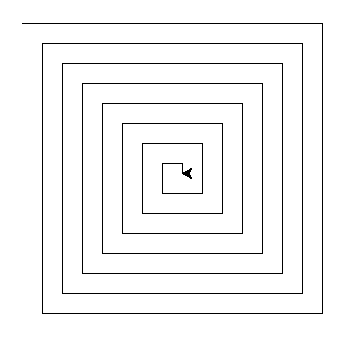
\includegraphics[width=0.3\textwidth]{fig/spirale.png}
    \caption{Une spirale}
    \label{fig:spirale}
  \end{figure}

  Pour dessiner une spirale de côté $c > 0$ :
  \begin{enumerate}
  \item On trace un trait de longueur $c$
  \item On tourne le stylo de $90$ degrés
  \item On trace une spirale de côté $c-d$, où $d$ est l'écart entre un côté de la spirale et le suivant.
  \end{enumerate}
  
\end{frame}

\begin{frame}
  \frametitle{Teaser : l'arbre d'Auto-Warhol}

  \begin{figure}[ht]
    \centering
    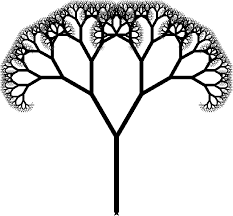
\includegraphics[width=0.5\textwidth]{fig/arbre.png}
    \caption{Un arbre}
    \label{fig:arbre}
  \end{figure}

\end{frame}

\begin{frame}[fragile]{Cas de base}
  \begin{block}{Fonction récursive}
    \vspace{0pt}
    \MVRightarrow{} Une fonction qui s'appelle elle-même.
  \end{block}

\begin{minted}{python}
def fact(n):
    return n * fact(n-1)
\end{minted}

  \pause

  \begin{alertblock}{Attention !}
    \vspace{0pt}
    Pour qu'elle termine, une fonction récursive doit avoir un ou plusieurs \emph{cas de base}. \newline
    (comme une boucle \mintinline{python}{while} doit avoir une condition d'arrêt)
  \end{alertblock}

\end{frame}

\begin{frame}[fragile]{Appels récursifs}

\begin{minted}{python}
def fact(n):
    if n == 0:
        return 1
    else:
        return n * fact(n)
\end{minted}

  \pause

  \begin{alertblock}{Attention !}
    \vspace{0pt}
    Pour qu'elle termine, une fonction récursive doit s'auto-appeler sur des arguments \emph{plus simples}. \newline
    (comme une boucle \mintinline{python}{while} qui dépend de \mintinline{python}{n} doit modifier \mintinline{python}{n}, sinon elle ne termine pas)
  \end{alertblock}

\end{frame}

\begin{frame}
  \frametitle{Exemple : l'arbre d'Auto-Warhol}

  \begin{figure}[ht]
    \centering
    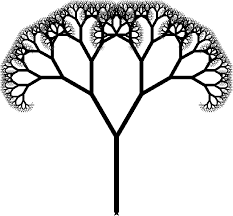
\includegraphics[width=0.5\textwidth]{fig/arbre.png}
    \caption{Un arbre}
    \label{fig:arbre}
  \end{figure}

\end{frame}

\begin{frame}
  \frametitle{Exemple : l'arbre d'Auto-Warhol}

  Pour dessiner un arbre dont le tronc mesure $L$ (si $L > 1$) :
  \begin{enumerate}
  \item On trace un trait de longueur $L$
  \item On tourne le stylo de $30$ degrés vers la gauche
  \item On trace un arbre de tronc $\dfrac{2}{3} L$
  \item On tourne le stylo de $30$ degrés vers la droite \newline pour le remettre en position
  \item On tourne le stylo de $30$ degrés vers la droite
  \item On trace un arbre de tronc $\dfrac{2}{3} L$
  \item On tourne le stylo de 30 degrés vers la gauche \newline pour le remettre en position
  \item On ramène le stylo à sa place en traçant un trait de longueur $L$ à l'envers
  \end{enumerate}
  
\end{frame}

\section{Suppléments sur les fonctions}

\begin{frame}{Fonctions}
    \begin{tikzpicture}
      % Rectangle pour représenter la fonction
      \node [draw, rectangle, text width=2cm, minimum height=1.5cm, align=center] (function) at (0,0) {Fonction};

      % Chemin pour représenter l'entrée (paramètres)
      \draw[-latex] (-5,0) -- (-1.2,0) node[midway, above, label={below: (paramètres)}] {Entrée};

      % Chemin pour représenter la sortie (valeur de retour)
      \draw[-latex] (1.2,0) -- (5,0) node[midway, above, label= {below: (valeur de retour)}] {Sortie};

      % Flèche d'affichage (zig-zag)
      \onslide<2->{\draw [decorate, -latex, decoration={snake, segment length=5mm, amplitude=1mm, post length=1mm}] (0,0.5) -- (0,2.5) node[pos = 0.75, right, label = {left:\small Effets de bord}] {\begin{tabular}{l}Afficher à l'écran \\ Écrire dans un fichier\end{tabular}};}

      % Flèche d'effets de bord (zig-zag)
      \onslide<3->{\draw [decorate, -latex, decoration={snake, segment length=5mm, amplitude=1mm, post length=1mm}] (0,-2.5) -- (0,-0.5) node[pos = 0.25, right, label = {left:\small Effets de bord}] {\begin{tabular}{l} Demander une entrée à l'utilisateur \\ Lire dans un fichier\end{tabular}};}
    \end{tikzpicture}
\end{frame}


\end{document}

%%% Local Variables:
%%% TeX-engine: xetex
%%% TeX-command-extra-options: "-shell-escape"
%%% End:
